
    %                     %            %
    %                                  %
    %                                  %
   %%%    %%%%   %%%%%   %%           %%%    %%%%  %    %
    %    %    % %         %            %    %    %  %  %
    %    %%%%%%  %%%%     %            %    %%%%%%   %%
    %    %           %    %            %    %        %%
    %    %           %    %     %%     %    %       %  %
     %%   %%%%% %%%%%    %%%    %%      %%   %%%%% %    %



         %%%%%%%%%%%%%%%%%%%%%%%%%%%%%%%%%%%%%%%%
         %                                      %
         %  "Scheletro" di una tesi di laurea   %
         %           (in Matematica)            %
         %      dell'Universita` di Udine       %
         %                                      %
         %%%%%%%%%%%%%%%%%%%%%%%%%%%%%%%%%%%%%%%%

              %%%%%%%%%%%%%%%%%%%%%%%%%%%%
              %  Autore: Gianluca Gorni  %
              %%%%%%%%%%%%%%%%%%%%%%%%%%%%

   %%%%%%%%%%%%%%%%%%%%%%%%%%%%%%%%%%%%%%%%%%%%%%%%%%%%%
   %%%%%   Ultima modifica:  27 febbraio 2013      %%%%%
   %%%%%%%%%%%%%%%%%%%%%%%%%%%%%%%%%%%%%%%%%%%%%%%%%%%%%



                                 %            %%
                                 %             %
   %%%%  % %%   %%%   %%%% %%%%  %%%%   %%%    %    %%%
   %   % %%  % %   % %   % % % % %   % %   %   %   %   %
   %   % %     %%%%% %   % % % % %   % %   %   %   %   %
   %   % %     %     %  %% % % % %   % %   %   %   %   %
   %%%%  %      %%%%  %% % % % % %%%%   %%%   %%%   %%%
   %
   %




  %%%%%%%%%%%%%%%%%%%%%%%%%%%%%%%%%%%%%%%%%%%%%%%%%%%%%%%%%
  % Usare una versione di LaTeX con sillabazione italiana %
  %%%%%%%%%%%%%%%%%%%%%%%%%%%%%%%%%%%%%%%%%%%%%%%%%%%%%%%%%

\documentclass[12pt,a4paper,twoside,english,italian]{book}

% Usare "oneside" invece di "twoside"
% nelle bozze, per risparmiare carta:
% "twoside" produce diverse pagine bianche
% alla fine dei capitoli.

                    %%%%%%%%%%%%%%%%%%%%%%%%%%%%%%%%
                    %         inputenc             %
                    %  Usare l'opzione "latin1"    %
                    %  se si vogliono scrivere     %
                    %  lettere accentate da        %
                    %  tastiera su Windows o Unix  %
                    %%%%%%%%%%%%%%%%%%%%%%%%%%%%%%%%

\usepackage[latin1]{inputenc}

       %%%%%%%%%%%%%%%%%%%%%%%%%%%%%%%%%%%%%%%%%%%%%%
       %                  babel                     %
       % Pacchetto tipico per una tesi in italiano. %
       %%%%%%%%%%%%%%%%%%%%%%%%%%%%%%%%%%%%%%%%%%%%%%


\usepackage{babel}


   %%%%%%%%%%%%%%%%%%%%%%%%%%%%%%%%%%%%%%%%%%%%%%%%%%%%%%%%%%%%
   % Se nella tesi si inseriscono dei passi in un'altra       %
   % lingua (inglese, per fissare le idee), si puo' istruire  %
   % il TeX di sillabare quella parte di testo con le regole  %
   % inglesi, invece che italiane. A questo scopo basta       %
   % scrivere                                                 %
   %                                                          %
   %    \documentclass[...,english,italian,...]{...}          %
   %                                                          %
   % al posto di \documentclass[...,italian,...],             %
   % dopodiche' la sillabazione sara' italiana fintanto che   %
   % non si incontra il comando \selectlanguage{english}.     %
   % Per tornare all'italiano si scrive                       %
   % \selectlanguage{italian}                                 %
   %%%%%%%%%%%%%%%%%%%%%%%%%%%%%%%%%%%%%%%%%%%%%%%%%%%%%%%%%%%%

\usepackage{uniudtesi}

% Col pacchetto tocbibind compariranno nell'indice anche
% la bibliografia ed eventualmente l'indice analitico
\usepackage[nottoc]{tocbibind}

% Il pacchetto indentfirst abolisce la fastidiosa convenzione
% anglosassone di fa cominciare la prima riga di un
% capitolo o sezione a margine sinistro, senza rientro:
\usepackage{indentfirst}

% \usepackage{graphicx} % gia' caricato da uniudtesi
\graphicspath{{./figure/}}
%\usepackage{epstopdf}

% Per l'ipertesto:
% \usepackage{hyperref} % gia' caricato da uniudtesi
\hypersetup{
  % pdfpagelayout=SinglePage, % default
  % pdfpagemode=UseOutlines, % default
  bookmarksopen, % default
  bookmarksopenlevel=2, % default;
  pdftitle={La mia Tesi},
  pdfauthor={Giovanna Tesista},
  pdfsubject={Modello di Tesi di Laurea},
  pdfkeywords={tesi laurea LaTeX}} % Queste informazioni non vengono stampate, ma sono conservate nel documento pdf. Sono consultabili col menu "File>Document Properites>Description". Vengono buone a scopi archivistici.
%%%%%%%%%%%%%%%%%%%%%%%%%%%%%%%%%%%%%%%%%%%%%%%%%%%%%%%%%%%%

       %%%%%%%%%%%%%%%%%%%%%%%%%%%%%%%%%%%%%%%%%%%%%%%%
       % Pacchetti tipici per una tesi di matematica  %
       %%%%%%%%%%%%%%%%%%%%%%%%%%%%%%%%%%%%%%%%%%%%%%%%

\usepackage{amsmath,amsfonts,amssymb,amsthm}
\usepackage{latexsym}


%%%%%%%%%%%%%%%%%%%%%%%%%%%%%%%%%%%%%%%%%%%%%%%%%%%%%%%
%                    graphicx                         %
%                                                     %
%   Uno dei pacchetti per l'inserzione di figure      %
%   in formato eps e` "graphicx". Ce ne sono diversi  %
%   altri da cui scegliere.                           %
%                                                     %
%   Esempio di uso: avendo un file di nome            %
%   figura1.eps questa si inserisce nella tesi        %
%   col comando                                       %
%                                                     %
%        \begin{figure}[ht]                           %
%        \begin{center}                               %
%        \includegraphics{figura1.eps}                %
%        \caption[nome breve]{nome lungo}             %
%        \label{etichetta}                            %
%        \end{center}                                 %
%        \end{figure}                                 %
%                                                     %
%   Il "nome breve" e` quello che apparira`           %
%   nell'indice delle figure ed e' opzionale.         %
%   Il "nome lungo" e' quello che appare              %
%   sotto la figura.                                  %
%   (Ci sono opzioni per scalare, spostare, ruotare   %
%   le figure).                                       %
%   Con \graphicspath{{./figure/}} si dice            %
%   al LaTeX di cercare le figure nella cartella      %
%   "figure" situata allo stesso livello di           %
%   questo documento                                  %
%                                                     %
%%%%%%%%%%%%%%%%%%%%%%%%%%%%%%%%%%%%%%%%%%%%%%%%%%%%%%%


   %%%%%%%%%%%%%%%%%%%%%%%%%%%%%%%%%%%%%%%%%%%
   %  Esempi di macro definite dall'utente.  %
   %  Le prime definiscono dei comandi per   %
   %  scrivere i caratteri speciali per      %
   %  gli insiemi numerici fondamentali      %
   %  (naturali, interi, razionali, reali,   %
   %  complessi                              %
   %%%%%%%%%%%%%%%%%%%%%%%%%%%%%%%%%%%%%%%%%%%

\newcommand{\N}{\mathbb{N}}
\newcommand{\Z}{\mathbb{Z}}
\newcommand{\Q}{\mathbb{Q}}
\newcommand{\R}{\mathbb{R}}
\newcommand{\C}{\mathbb{C}}

   %%%%%%%%%%%%%%%%%%%%%%%%%%%%%%%%%%%%%%%%%%%%
   %  Delle macro che definiscono operatori   %
   %  non predefiniti in LaTeX. Ogni utente   %
   %  aggiunge quelle che servono. Questi     %
   %  sono solo esempi arbitrari.             %
   %%%%%%%%%%%%%%%%%%%%%%%%%%%%%%%%%%%%%%%%%%%%

\DeclareMathOperator{\traccia}{tr}
\DeclareMathOperator{\sen}{sen}
\DeclareMathOperator{\arcsen}{arcsen}
\DeclareMathOperator*{\maxlim}{max\,lim}
\DeclareMathOperator*{\minlim}{min\,lim}
\DeclareMathOperator*{\deepinf}{\phantom{\makebox[0pt]{p}}inf}

    %%%%%%%%%%%%%%%%%%%%%%%%%%%%%%%%%%%%%%%%%%%%
    % Esempi di macro piu` elaborate,          %
    % contenenti degli argomenti.              %
    % Compongono gli indici delle sommatorie   %
    % e delle produttorie in modo diverso      %
    % da quello standard del TeX. Dovrebbero   %
    % funzionare bene quando gli estremi della %
    % sommatoria sono piccoli. Chi volesse     %
    % usarle estesamente farebbe bene a        %
    % lavorarci sopra.                         %
    %%%%%%%%%%%%%%%%%%%%%%%%%%%%%%%%%%%%%%%%%%%%

\newcommand{\varsum}[3]{\sum_{#2}^{#3}\!
   {\vphantom{\sum}}_{#1}\;}
\newcommand{\varprod}[3]{\sum_{#2}^{#3}\!
   {\vphantom{\sum}}_{#1}\;}

  %%%%%%%%%%%%%%%%%%%%%%%%%%%%%%%%%%%%%%%%%%%%%%%%%%%%%%%
  %          Numerazione delle formule                  %
  % Se non specificato altrimenti, il LaTeX numera le   %
  % formule come (capitolo.formula) (per esempio (2.5)  %
  % e` la quinta formula del secondo capitolo).         %
  % Con le istruzioni seguenti invece la numerazione    %
  % diventa (capitolo.sezione.formula) (per esempio     %
  % (3.2.6) e` la sesta formula della seconda sezione   %
  % del terzo capitolo):                                %
  %%%%%%%%%%%%%%%%%%%%%%%%%%%%%%%%%%%%%%%%%%%%%%%%%%%%%%%

%\makeatletter
%\@addtoreset{equation}{section}
%\makeatother
%\renewcommand{\theequation}%
%  {\thesection.\arabic{equation}}


              %%%%%%%%%%%%%%%%%%%%%%%%%%
              % Stile degli enunciati  %
              %%%%%%%%%%%%%%%%%%%%%%%%%%

%%%%%%%%%%%%%%%%%%%%%%%%%%%%%%%%%%%%%%%%%%%%%%%%%%%%%%%%%%%
% Con le dichiarazioni seguenti                           %
% teoremi, definizioni, proposizioni, lemmi e corollari   %
% vengono numerati capitolo per capitolo e con un         %
% contatore unico per tutti (per esempio, se subito dopo  %
% il Teorema 2.1 c'e' una definizione, questa sara'       %
% Definizione 2.2)                                        %
%%%%%%%%%%%%%%%%%%%%%%%%%%%%%%%%%%%%%%%%%%%%%%%%%%%%%%%%%%%

\theoremstyle{plain}
\newtheorem{teorema}{Teorema}[chapter]
\newtheorem{proposizione}[teorema]{Proposizione}
\newtheorem{lemma}[teorema]{Lemma}
\newtheorem{corollario}[teorema]{Corollario}

\theoremstyle{definition}
\newtheorem{definizione}[teorema]{Definizione}
\newtheorem{esempio}[teorema]{Esempio}

\theoremstyle{remark}
\newtheorem{osservazione}[teorema]{Osservazione}

  %%%%%%%%%%%%%%%%%%%%%%%%%%%%%%%%%%%%%%%%%%%%%%%%%%%%%%%%
  % I comandi si usano cosi`:                            %
  %                                                      %
  %   \begin{teorema}[di Pitagora]                       %
  %   La somma dei quadrati ecc.                         %
  %   \end{teorema}                                      %
  %                                                      %
  % Le parole "di Pitagora" fra parentesi quadre         %
  % sono facoltative. Non bisogna inserire               %
  % manualmente degli spazi prima e dopo gli enunciati,  %
  % perche' e` automatico!                               %
  %%%%%%%%%%%%%%%%%%%%%%%%%%%%%%%%%%%%%%%%%%%%%%%%%%%%%%%%


  %%%%%%%%%%%%%%%%%%%%%%%%%%%%%%%%%%%%%%%%%%%%%%%%%%%%%%%%%%%%%%
  % Il pacchetto amsthm definisce anche l'ambiente "proof"     %
  % per le dimostrazioni.                                      %
  % Esempio di uso:                                            %
  %                                                            %
  %   \begin{proof}                                            %
  %   Sia $X$ un insieme ecc.                                  %
  %   \end{proof}                                              %
  %                                                            %
  %%%%%%%%%%%%%%%%%%%%%%%%%%%%%%%%%%%%%%%%%%%%%%%%%%%%%%%%%%%%%%

       %%%%%%%%%%%%%%%%%%%%%%%%%%%%%%%%%%%%%%%%%%%%%%%%%%%%%%%
       %                   makeidx                           %
       %                                                     %
       % Pacchetto per la generazione automatica dell'indice %
       % analitico. Per esempio, se vogliamo che la parola   %
       % "analitico" venga indicizzata nella frase           %
       %                                                     %
       %    "un metodo analitico di soluzione"               %
       %                                                     %
       % bisogna scrivere                                    %
       %                                                     %
       %    "un metodo analitico\index{analitico} di         %
       %              soluzione".                            %
       %                                                     %
       % Compilando il file, il LaTeX produrra' un file      %
       % ausiliario che termina con ".idx". Bisogna far      %
       % processare questo file idx dal programma            %
       % ausiliario "bibtex", che produrra' a sua volta un   %
       % altro file ancora. Dare infine un'ultima passata    %
       % col LaTeX. Si puo' tranquillamente lasciare         %
       % la compilazione dell'indice verso la fine della     %
       % stesura del lavoro, quando tutto e' ormai quasi     %
       % definitivo.                                         %
       %                                                     %
       %%%%%%%%%%%%%%%%%%%%%%%%%%%%%%%%%%%%%%%%%%%%%%%%%%%%%%%

%\usepackage{makeidx}
%\makeindex

% Ridefiniamo la riga di testa delle pagine:
\usepackage{fancyhdr}
\pagestyle{fancy}
\renewcommand{\chaptermark}[1]{\markboth{#1}{}}
\renewcommand{\sectionmark}[1]{\markright{\thesection\ #1}}
\fancyhf{}
\fancyhead[LE,RO]{\bfseries\thepage}
\fancyhead[LO]{\bfseries\rightmark}
\fancyhead[RE]{\bfseries\leftmark}
\renewcommand{\headrulewidth}{0.5pt}
\renewcommand{\footrulewidth}{0pt}
\setlength{\headheight}{14.5pt}

               %%%%%%%%%%%%%%%%%%%%%%%%%%%%%%%%%%%%%%
               %  Informazioni generali sulla Tesi  %
               %    da usare nell'intestazione      %
               %%%%%%%%%%%%%%%%%%%%%%%%%%%%%%%%%%%%%%

  \titolo{La mia tesi\\ di Matematica}
  \laureanda{Giovanna Tesista}
% \laureando{Giovanni Tesista}
  \annoaccademico{2012-2013}
% \facolta{Scienze Matematiche, Fisiche e Naturali} % (default)
%  \corsodilaurea{Informatica} % per la laurea vecchio ordinamento
%\corsodilaureatriennalein{Matematica}
% \corsodilaureaspecialisticain{Informatica}
 \corsodilaureamagistralein{Matematica}
  \relatore[Prof.]{Tal dei Tali}
% \correlatore{Talaltro dei Tali}
% \correlatoreDue{Secondo Correlatore}
  \dedica{Ai miei genitori\\
    per non avermi tagliato i viveri} % (facoltativo)


   %%%                                    %        %%    %%
  %   %                                   %         %     %
  %      %%%  % %%  %%%%   %%%         %%%%  %%%    %     %    %%%%
  %     %   % %%  % %   % %   %       %   % %   %   %     %   %   %
  %     %   % %     %   % %   %       %   % %%%%%   %     %   %   %
  %   % %   % %     %   % %   %       %   % %       %     %   %  %%
   %%%   %%%  %     %%%%   %%%         %%%%  %%%%  %%%   %%%   %% %
                    %
                    %


                          %%%%%               %
                            %
                            %    %%%   %%%%  %%
                            %   %   % %       %
                            %   %%%%%  %%%    %
                            %   %         %   %
                            %    %%%% %%%%   %%%


 \begin{document}

         %%%%%%%%%%%%%%%%%%%%%%%%%%%%%%%%%%%%%%%%%%%%%%%%%
         %            Intestazione                       %
         %                                               %
         % Per l'intestazione completa bisogna           %
         % essersi procurati il file "polloPallido.eps". %
         %%%%%%%%%%%%%%%%%%%%%%%%%%%%%%%%%%%%%%%%%%%%%%%%%

\frontmatter
\maketitle

  %%%%%%%%%%%%%%%%%%%%%%%%%%%%%%%%%%%%%%%%%%%%%%%%%%%%%%%%%%%
  %   Si puo` scegliere fra scrivere tutta la tesi in un    %
  %   solo file, oppure distribuire ogni capitolo in un     %
  %   file a parte. Qui si e` scelto tenere separati i      %
  %   vari capitoli, che vengono caricati con \include      %
  %%%%%%%%%%%%%%%%%%%%%%%%%%%%%%%%%%%%%%%%%%%%%%%%%%%%%%%%%%%

\renewcommand{\theequation}{\arabic{equation}}%consigliato per migliorare i numeri di equazione nell'introduzione
\renewcommand{\thesection}{\arabic{section}}%consigliato per migliorare i numeri di equazione nell'introduzione

       %%%%%%%%%%%%%%%%%%%%%%
       %                    %
       %  Introduzione.tex  %
       %                    %
       %%%%%%%%%%%%%%%%%%%%%%

\chapter{Introduzione}

Il \TeX{} fu pensato ai lontani tempi in cui i terminali
grafici erano un lusso stravagante e l'unico modo di
comunicare coi calcolatori era di battere tasti della
tastiera. Ancora oggi chi scrive in \TeX{} deve inserire i
comandi di formattazione mescolati al testo ed \`e meglio
se ha un manuale a portata di mano. Per rialzare
il morale basta che si rammenti che il \TeX{} \`e ancora
solidamente il pi\`u sofisticato sistema di impaginazione
per testi scientifici, e che \`e gratis.

\section{Prima sezione}

Per cominciare a scrivere in \TeX{} bisogna individuare i
\emph{caratteri speciali}, o \emph{caratteri di
controllo}\index{caratteri di controllo}, che servono a
distinguere il testo dai comandi. Chi lavora con la
tastiera italiana\index{tastiera italiana} dovr\`a faticare
all'inizio, perch\'e alcuni di quei caratteri importanti
si raggiungono solo attraverso certe combinazioni di
tasti, che per di pi\`u cambiano da un sistema
operativo\index{sistema operativo} a un altro. Consultate
il manuale del vostro calcolatore o chiedete aiuto agli
esperti se non vi raccapezzate.

Questa \`e un'equazione numerata:
\begin{equation}\label{prodottoNotevole}
  (a-b)(a+b)=a^2-b^2.
\end{equation}
Notate il numero di equazione al margine destro. Ne riparleremo nel prossimo capitolo. Notate anche il numero di sezione. In questo esempio di tesi, le sezioni dell'introduzione sono numerate con un singolo numero, mentre nei capitoli seguenti\dots\ beh, guardate voi stessi.

\begin{itemize}

\item Il carattere speciale principe del \TeX{} \`e il
\verb!\!, chiamato \emph{``backslash''}
\index{backslash (\verb?\?)}
(che significa grosso modo ``fendente inverso'', da non
confondere con~\verb!/!, che \`e lo ``slash'', o linea di
frazione), che serve per annunciare i comandi. Vi conviene
imparare subito il suo posto sulla tastiera. Come carattere
coincide con il segno meno della teoria degli insiemi
($A\setminus B$)\index{sottrazione insiemistica}, che
per\`o si raccomanda di ricavare col comando
\verb!\setminus!.

\item Le \emph{parentesi
graffe}~\verb!{}!\index{parentesi graffe} sono pure
fondamentali e vanno individuate subito sulla tastiera.
Servono per delimitare le zone di azione di un comando.
Quando le graffe vanno stampate, come nella formula
$\{a\}$, basta farle precedere dal backslash:
\verb!\{a\}!.

\item Il segno del \emph{dollaro}~\$ \index{dollaro,
simbolo del} serve per delimitare le formule inglobate nel
testo. Ad esempio per ottenere $A\setminus B$ scriviamo
\verb!$A\setminus B$!.

\item Gli \emph{accenti}\index{accenti} \verb!`! e \verb!'!
preceduti da backslash servono per accentare il carattere
che segue: per ottenere \`{a}, \`{e}, \'{e}, \`{u} si batte
\verb!\`{a}!, \verb!\`{e}!, \verb!\'{e}!, \verb!\`{u}!. Addirittura
la~\`{\i} accentata \`e patologicamente complicata: si
ottiene battendo \verb!\`{\i}!. Se trovate farraginoso
questo metodo di scrivere le lettere accentate, non siete
gli unici. Per questo viene in aiuto il pacchetto
``\verb!inputenc!'', che viene caricato col comando \begin{center}\verb!\usepackage[latin1]{inputenc}!\end{center} (su windows o unix)\index{accenti su windows o unix}.
Con questo pacchetto attivo il \LaTeX{} interpreta
correttamente gli accenti da tastiera �, �, �, ecc.
Il backslash rimane per gli accenti e segni diacritici
\index{accenti stranieri}
non italiani: \verb!\^{o}! per l'H\^{o}pital,
\verb!\"{o}! per G\"odel, \verb!\~{n}!
per Espa\~{n}a, \verb!\c{c}! per gar\c{c}on, ecc.
Battendo due volte gli accenti, come in
\verb!``virgolette''! si ottengono le
``virgolette''\index{virgolette} aperte e chiuse.

\item Il \emph{percento}~\verb!%!\index{percento, segno
del} dice al \TeX{} di ignorare il resto della riga di
input, per inserire ``commenti'' al testo sorgente che non
andranno stampati.

\item Il \emph{``cappuccio''}~\verb!^!
\index{cappuccio (\verb?^?)} e
la \emph{sottolineatura}~\verb!_!\index{sottolineatura},
che servono soprattutto per gli esponenti e gli indici
nelle formule: per avere
$a_i^2$ battere \verb!$a_i^2$!, o, indifferentemente
\verb!$a^2_i$!.

\item Le \emph{parentesi
quadre}~\verb![]!\index{parentesi quadre} e i segni di
\emph{disuguaglianza}~$<>$ servono nelle formule
matematiche e in certe tastiere sono nascosti.

\item L'\emph{``ampersand''}\index{ampersand (\verb?&?)}, o
``e~commerciale''~\verb!&!, che separa gli argomenti di un
allineamento.

\item La
\emph{``tilde''}~\verb!~!\index{tilde (\verb?~?)},
che posta fra due parole vieta al \TeX{} di andare a capo
in quel punto. Per esempio scriveremo
\verb!Prof.~Tizio! se siamo pignoli e non vogliamo che
``Prof.'' c\`{a}piti a fine riga e ``Tizio'' sia spedito a
capo. L'accento tilde sulla lettera seguente (come in
Espa\~{n}a o S\~{a}o Paulo) si ottiene con~\verb!\~!
(\verb!Espa\~{n}a!,
\verb!S\~{a}o Paulo!). La tilde nelle formule matematiche
\`e diversa: per avere $\tilde a$ bisogna battere
\verb!$\tilde a$!.

\item Lo
\emph{``hash''}~\verb!#!\index{hash (\verb?#?)}
serve come segnaposto per gli argomenti delle funzioni.
Troppo complicato da spiegare qui.

\end{itemize}

\tableofcontents
\listoffigures

\mainmatter

\renewcommand{\theequation}{\thechapter.\arabic{equation}}%si torna alle formule numerate come da default
\renewcommand{\thesection}{\thechapter.\arabic{section}}%si torna alle sezioni numerate come da default

     %%%%%%%%%%%%%%%%%%%%
     %                  %
     %  capitolo1.tex   %
     %                  %
     %%%%%%%%%%%%%%%%%%%%

\chapter{Rudimenti di \TeX}

Raccogliamo qui alcune delle cose di base per un
principiante di \TeX.

\section{Spazi}

Uno o pi\`u spazi fra due parole del testo sorgente non
fanno differenza: \verb!uno due! ha lo stesso effetto
di \verb!uno     due!. Per terminare il
paragrafo e avere il rientro nella riga seguente il modo
consigliato \`e di lasciare una o pi\`u righe bianche dopo
la fine del paragrafo. Un'alternativa \`e di scrivere
\verb!\par! alla fine del paragrafo.

Un'altra equazione numerata:
\begin{equation}\label{prodottoNotevole2}
  (a-b)(a^2+ab+b^2)=a^3-b^3.
\end{equation}

La spaziatura verticale \`e gestita in gran parte
automaticamente dal \LaTeX. Se si vuole uno stacco \`e
spesso meglio vedere se non sia il caso di introdurre una
nuova \verb!\section!, \verb!\subsection!
\verb!\subsubsection!, \verb!itemize! o un enunciato
(\verb!osservazione!, \verb!corollario! ecc.), e fidarsi
della spaziatura automatica.

Se proprio si vuole inserire uno spazio manualmente si
pu\`o usare il comando
\verb!\hspace{!\textit{lunghezza}\verb!}! per gli spazi
orizzontali e \verb!\vspace{!\textit{lunghezza}\verb!}!
per gli spazi verticali. Per esempio scrivendo
\begin{center}
  \verb!\hspace{1cm}!
\end{center}
si lascia uno spazio orizzontale di 1 centimetro.
Per gli spazi verticali \`e meglio scegliere fra i
seguenti tre spazi standardizzati piccolo, medio e grande:
\begin{center}
  \verb!\smallskip!, \verb!\medskip!, \verb!\bigskip!.
\end{center}

\section{Trattini}

Il \TeX{} distingue quattro tipi di trattini
orizzontali. Notate come sono diversi per lunghezza,
spessore e spaziatura.

\begin{itemize}

\item il trattino semplice (esempio:
video-proiettore), che si ottiene battendo il tasto del
trattino (o~segno meno): \verb!video-proiettore!.

\item il trattino medio, che per quanto ne so si usa
solo fra due numeri per indicare l'intervallo fra i due,
per esempio nel citare le pagine da 15 a 21 di un libro
potr\`o scrivere ``p.~15--21''. Questo trattino si
ottiene battendo due volte il tasto del trattino semplice:
\verb!p. 15--21!.

\item il trattino lungo, poco usato in italiano, ma che
in inglese \`e spesso usato per delimitare un
inciso---come noi useremmo una parentesi. Si ottiene
battendo tre volte il trattino semplice:
\verb!inciso---come!. Nella tipografia inglese non si
lasciano spazi attorno al trattino lungo.

\item il segno meno, che si usa nelle formule
matematiche: $a-1$. Si ottiene battendo il trattino
semplice, ma all'interno di una formula: \verb!$a-1$!.
Qui i dollari servono per delimitare la formula.

\end{itemize}

Un'altra equazione numerata:
\begin{equation}
  (a-b)(a^3+a^2b+ab^2+b^3)=a^4-b^4.
\end{equation}
Per come \`e settato questo esempio di tesi, il numero di equazione \`e una coppia il cui primo elemento \`e il numero di capitolo e il secondo \`e il numero di formula all'interno del capitolo. Per esempio, nella formula~\eqref{prodottoNotevole2} di pag.~\pageref{prodottoNotevole2} il primo~`1' si riferisce al capitolo (non alla sezione!) e il secondo~`1' alla formula. Fanno eccezione le formule dell'introduzione, il cui numero non \`e una coppia ma un singolo numero d'ordine (vedi la formula~\eqref{prodottoNotevole} di pag.~\pageref{prodottoNotevole}).


\section{Accenti, lettere insolite, e cambi di font}

Alcuni esempi di lettere o accenti stranieri:
\begin{center}
\begin{tabular}{ll}
  Weierstra\ss & \verb!Weierstra\ss! \\
  G\"odel & \verb!G\"odel! \\
  na\"{\i}ve & \verb!na\"{\i}ve! \\
   {\O}ystein & \verb!{\O}ystein! \\
  {\AA}ngstr\"om & \verb!{\AA}ngstr\"om! \\
  Stanis{\l}aw \'Swierczkowski & 
    \verb!Stanis{\l}aw \'Swierczkowski! \\
  P\'al Erd\H{o}s &
    \verb!P\'al Erd\H{o}s! \\
  T\=oky\=o & \verb!T\=oky\=o! \\
  L'H\^opital & \verb!L'H\^opital!
\end{tabular}
\end{center}
Se ve ne servono degli altri consultate un manuale.

\medskip

Varie \emph{forme} dei caratteri e i comandi per
ottenerle:

\medskip

\begin{center}
\begin{tabular}{ll}
  \textup{Testo normale (upright)} &
    \verb!\textup{Testo normale!\\
    &\qquad\verb!(upright)}!\\ 
  \textit{corsivo (``italic'')} &
    \verb!\textit{corsivo!\\
    &\qquad\verb!(``italic'')}!\\
  \textsl{inclinato (``slanted'')} &
    \verb!\textsl{inclinato!\\
    &\qquad\verb!(``slanted'')}!\\
  \textsc{maiuscolette (``small caps'')} &
    \verb!\textsc{maiuscolette!\\
    &\qquad\verb!(``small caps'')}!
\end{tabular}
\end{center}
%
Varie \emph{serie} (o pesantezza) di caratteri:
%
\begin{center}
\begin{tabular}{ll}
  \textmd{serie media (normale)} &
    \verb!\textmd{serie media!\\
    &\qquad\verb!(normale)}!\\
  \textbf{serie grassetta (``boldface'')} &
    \verb!\textbf{grassetto!\\
    &\qquad\verb!(``boldface'')}!
\end{tabular}
\end{center}
%
Varie \emph{famiglie} di caratteri:
%
\begin{center}
\begin{tabular}{ll}
  \textrm{famiglia romana (normale)} &
    \verb!\textrm{famiglia romana!\\
    &\qquad\verb!(normale)}!\\
  \textsf{senza grazie (``sans serif'')} &
    \verb!\textsf{senza grazie!\\
    &\qquad\verb!(``sans serif'')}!\\
  \texttt{telescrivente (``typewriter'')}&
    \verb!\texttt{telescrivente!\\
    &\qquad\verb!(``typewriter'')}!
\end{tabular}
\end{center}
%
Forme, serie e famiglie si possono combinare: battendo
\begin{center}
  \verb!\textsf{\textbf{Cosa?}}!
\end{center}
si ottiene \textsf{\textbf{Cosa?}} Non tutte le
combinazioni per\`o sono supportate.

Attenzione! Una tesi di laurea non \`e il luogo per
sbizzarrirsi con l'uso di caratteri strani. La parola
d'ordine \`e \emph{sobriet\`a} e da evitare sono le
\emph{pacchianate}. Normalmente non avrete bisogno di
altro che di evidenziare qualche parola qua e l\`a nel
testo, e per questo si raccomanda di usare il comando
\verb!\emph!. Per esempio per produrre
\emph{testo enfatico} basta battere
\verb!\emph{testo enfatico}! e lasciare il resto al
\LaTeX.

Chi deve inserire nel testo dei listati di programmi di
calcolatore, si veda i manuali riguardo i comandi
\verb!\verb!, \verb!\verbatim! e i pacchetti
\verb!verbatim!, \verb!moreverb! e simili.

Il pacchetto \verb!hyperref!,\index{ipertesto} (chiamato automaticamente da \verb!uniudtesi!, agevola i riferimenti a internet:

\begin{itemize}

\item gestisce automaticamente i font adatti, e 

\item rende ``cliccabili'' i riferimenti nelle versioni su schermo (dvi o pdf).

\end{itemize}

\noindent Per esempio, scrivendo \verb!\url{http://www.dimi.uniud.it}! viene

\begin{center}
\url{http://www.dimi.uniud.it}
\end{center}

   %%%%%%%%%%%%%%%%%%%
   %                 %
   %  capitolo2.tex  %
   %                 %
   %%%%%%%%%%%%%%%%%%%

\chapter{Enunciati e figure}
  
Il primo paragrafo dei capitoli non ha il rientro.

Gli altri paragrafi hanno il rientro.

\section{Enunciati}

Ora seguono due enunciati\index{enunciati}, in carattere inclinato, che condividono la numerazione\index{enunciati, numerazione degli} progressiva. Notare che la spaziatura \`e automatica!

\begin{teorema}[di Pitagora\index{Pitagora, teorema di}]
Il quadrato costruito sull'ipotenusa\index{ipotenusa} \`e uguale alla somma dei quadrati costruiti sui cateti\index{cateti}.
\end{teorema}

\begin{proof}
Si osservi la figura~\ref{figura:pitagora} a pagina~\pageref{figura:pitagora} (nel file \texttt{pdf} i riferimenti sono cliccabili\index{ipertesto}). Il~\LaTeX{} ha un suo modo di decidere se mettere la figura\index{figure, posizionamento delle} subito di seguito o spedirla in fondo alla pagina corrente o in cima alla pagina dopo, a seconda di quanto grande \`e la figura e di quanto spazio c'\`e.

\begin{figure}
\begin{center}
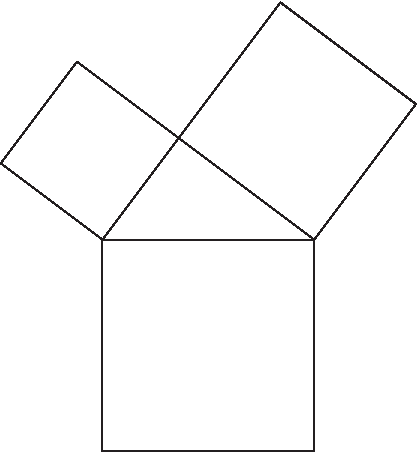
\includegraphics[width=200pt]{pitagora}
\caption[teor. di Pitagora]{Triangolo rettangolo}
\label{figura:pitagora}
\end{center}
\end{figure}

Esistono anche modi per far girare i testo attorno alle
figure. Chi vuole consulti i manuali.

Osservate comunque che in questo stile i paragrafi nelle dimostrazioni non hanno rientro\index{paragrafi, rientro dei} e c'\`{e} un quadratino\index{dimostrazioni, quadratino di fine} alla fine.
\end{proof}

\begin{definizione}\label{def:liminfinito}
Si dice che la successione reale $x_n$ tende\index{limite di successioni}\index{successioni, limite di} a~$+\infty$ se per ogni~$M\in\R$ esiste $n_M\in\N$ tale che per ogni~$n\ge n_M$ si ha che $x_n\ge M$.
\end{definizione}

Possiamo riferirci alla definizione~\ref{def:liminfinito}
tramite la sua etichetta\index{etichette}. Il riferimento sar\`{a} ``cliccabile'' se si \`{e} caricato il pacchetto \verb!uniudtesi! (il quale chiama a sua volta \verb!hyperref!.\index{ipertesto})

\section{Formule}

Anche le formule si possono etichettare:
\begin{equation}
  \label{eq:binomio}
  a+b\,.
\end{equation}
La formula precedente dovrebbe essere la~\ref{eq:binomio} (cliccabile). Non \`e obbligatorio numerare tutte le formule. Le formule non numerate\index{numerazione formule}\index{formule, numerazione delle}\index{numerazione delle formule} si ottengono o con doppi dollari\index{dollari, doppi}:
$$\dot x\quad
  \ddot x\quad
  \dddot x\quad
  \ddddot x$$
o con l'asterisco\index{asterisco}:
\begin{equation*}
  \overset{\circ}{A}\quad
  \overset{*}{X}\quad
  \vec{x}
\end{equation*}
Testo\index{formula, testo nella}\index{testo nella formula} mescolato a una formula:
\begin{equation}
  x+y=1\text{ quindi }(x+y)^2=1
\end{equation}
$$(x+y)^2\ge0\quad\text{ per ogni }x,y\in\R$$
Carattere grassetto\index{grassetto matematico} matematico:
$$\boldsymbol{y}
  $$
Allineamento\index{allineamento delle formule}\index{formule, allineamento delle} di formule e tre modi di indicare la congruenza\index{congruenze} modulo~$n^2$, con la seconda e terza formula numerate\index{formule, numerazione delle}\index{numerazione delle formule}:
\begin{align}
     u & \equiv  v+1 \pmod{n!}\nonumber \\
     u & \equiv v+1 \mod{n^2} \\
     u & \equiv v+1 \pod{n^2}
  \end{align}
Una formula spezzata\index{formula, spezzamento su righe diverse}\index{spezzamento di una formula su righe diverse} su due righe, ma trattata come un tutt'uno per il numero\index{formule, numerazione delle}\index{numerazione delle formule} di formula:
\begin{equation}
  \begin{split}
    f(x)  :={}& \int_0^{+\infty}t^{x-1}e^{-t}\,dt+\\
         &{}+e^{-x}
  \end{split}
\end{equation}
Due modi di scrivere le frazioni\index{frazioni}:
\begin{equation}
  \frac{1}{2}
  \quad\frac{1}{2}\,.
  \end{equation}
Una definizione per casi\index{casi, definizione
per}\index{definizione per casi}:
\begin{equation}
  f(x):=
  \begin{cases}
    x^2 & \text{se } x\ge0 \\
   -x^2 & \text{se }x<0
  \end{cases}
\end{equation}
Matrici\index{matrici} con e senza parentesi\index{parentesi}:
\begin{equation*}
  \begin{matrix}
    0 & 1 \\
    1 & 0
  \end{matrix}\quad
  \begin{pmatrix}
    0 & 1 \\
    1 & 0
  \end{pmatrix}
  \quad
  \begin{vmatrix}
    0 & 1 \\
    1 & 0
  \end{vmatrix}
\end{equation*}
Due formule di seguito senza allineamento\index{formule, allineamento delle}\index{allineamento delle formule}:
\begin{gather}
  (a+b)^2=a^2+2ab+b^2\label{eq:quadrato} \\
  (a+b)(a-b)(a^2+b^2)=a^4-b^4
\end{gather}

Un esempio di tavola\index{tavola}:

\begin{center}
\begin{tabular}{||l|lr||} \hline
gnats & gram & \$13.65 \\ \cline{2-3}
      & each &      .01 \\ \hline
gnu   & stuffed & 92.50 \\
    \cline{3-3}
emu   &      & 33.33 \\ \hline
armadillo & frozen & 8.99 \\ \hline
\end{tabular}
\end{center}

\appendix

\chapter{Come si fanno le appendici}
  
    \index{appendici}
    
    Le appendici si fanno con \verb!\appendix! seguito da
    \verb!\chapter{...}!

%%%%%%%%%%%%%%%%%%%%%%

\chapter{Esempi di Citazioni Bibliografiche}
  
    \index{bibliografia}
    \index{citazioni}
    
    P\^{y}r{\l}\aa{} in~\cite{pyrl} ha poi
    generalizzato i risultati di
    Bi\v{s}ker~\cite{bisker1}.
    
    Il pacchetto \verb!uniudtesi! carica
    automaticamente \verb!hyperref!\index{ipertesto},
    che a sua volta rende ``cliccabili'' i riferimenti 
    bibliografici nel documento elettronico.

%%%%%%%%%%%%%%%%%%%%%%

\chapter{Ambiente GNU/Linux (ad esempio Ubuntu)}

    \index{Linux}
    
    \begin{flushright}Contributo di\\ Leonardo Taglialegne
    \end{flushright}
    
    Gli ambienti GNU/Linux contengono parecchi strumenti utili per
    la stesura di una tesi di laurea, in particolare segnaliamo:
    \begin{itemize}
     \item Kile
     \item KBibTeX
    \end{itemize}
    Il primo \`e un editor per il \LaTeX, che include una tabella
    dei simboli, la visualizzazione della struttura, evidenziazione
    del codice e simili comodit\`a, e nelle ultime versioni fornisce
    una visualizzazione in anteprima dei risultati di compilazione.
    
    Il secondo \`e uno strumento di ricerca, modifica ed inserimento
    di citazioni in formato BibTeX.
    
    I pacchetti relativi (ed altri utili) si installano,
    su ambienti Debian e Ubuntu con:
    \texttt{sudo apt-get install kile kile-l10n kbibtex
           texlive-science \\
           texlive-math-extra texlive-lang-italian }


\backmatter

\begin{thebibliography}{10}

\frenchspacing

\bibitem{bisker1}
J. Bi\v{s}ker, \emph{On the elements
of the empty set}. Mathematica Absurdica
\textbf{132} (1999), 13--113.

\bibitem{pyrl}
U. P\^{y}r{\l}\aa, \emph{Generalization
of Bi\v{s}ker's theorem}. Paperopolis
J. Math. \textbf{14} (2001), 125--132.

\end{thebibliography}


% \printindex % se si fa l'indice analitico.

\end{document}
